\documentclass{beamer} 
\usetheme{Hannover}
\usepackage{amsmath}
\usepackage{amsfonts}
\usepackage{amssymb}
\usepackage{graphicx}
\usepackage{wasysym}
\usepackage{comment}

\newcommand{\eps}{\varepsilon}
\newcommand{\inner}[1]{\left\langle #1 \right\rangle}
\newcommand{\abs}[1]{\left| #1 \right|}
\newcommand{\norm}[1]{\left\| #1 \right\|}
\newcommand{\wt}{\widetilde}
\newcommand{\tbf}{\textbf}
\newcommand{\R}{\mathbb{R}}
\newcommand{\C}{\mathbb{C}}
\newcommand{\Q}{\mathbb{Q}}
\newcommand{\Z}{\mathbb{Z}}
\newcommand{\N}{\mathbb{N}}
\renewcommand{\P}{\mathbb{P}}
\newcommand{\E}{\mathbb{E}}

\title{From Calculus to Machine Learning} 
\author{Paul Siegel}

\begin{document} 
\frame{\titlepage}

\frame{
    What do linear regression, maximum likelihood estimation, support vector machines, and neural networks have in common? \pause

    \bigskip

    All fit into the following framework: \pause
    \begin{itemize}
        \item Identify a space of ``reasonable'' models \pause
        \item Construct a function which computes how well a given model fits the data \pause
        \item Find the model(s) which maximize (or minimize) the function
    \end{itemize}
}

\frame{
    Data scientists play a significant role in this process: \pause
    \begin{itemize}
        \item Identifying reasonable models uses domain expertise \pause
        \item Constructing a good objective function usually uses statistics \pause
        \item Finding the extremal model(s) uses math and/or engineering \pause
    \end{itemize}

    \bigskip

    In this seminar we'll try to understand some of the theory behind all three steps.
}

\frame{
    The plan:
    \begin{enumerate}
        \item Optimization for functions of one variable
        \item Linear algebra and PCA
        \item Optimization for functions of several variables
        \item Conditional probability and Bayesian statistics
        \item Linear regression
        \item Perceptrons
        \item Back propagation and gradient descent
    \end{enumerate}
}

\frame{
    \frametitle{1.1 Optimizing quadratic functions of one variable}
    You wish to build a rectangular fence next to a river.
    You have 100m of fence to work with and you want to enclose as much area as possible.
    How do you do it?
}

\frame{
    What is the space of models? \pause

    \bigskip

    \begin{itemize}
        \item Each possible fence is determined by its height $x$ and its width $y$ \pause
        \item Constraints: $x \geq 0$, $y \geq 0$, and $2x + y = 100$
    \end{itemize}
}

\frame{
    What is the objective function? \pause

    \bigskip

    We want to maximize the area $A(x,y) = xy$
}

\frame{
    This is now just a math problem: maximize $A(x,y) = xy$ subject to the constraints $x \geq 0$, $y \geq 0$, and $2x + y = 100$ \pause

    \bigskip

    This is an example of a \textit{constrained optimization} problem. \pause

    \bigskip 

    The objective function is quadratic and the constraint is linear, so we can hope to solve it analytically.
}

\frame{
    Using the constraint, eliminate $y$ to get:

    $$A(x) = x(100 - 2x)$$ \pause

    \begin{center}
        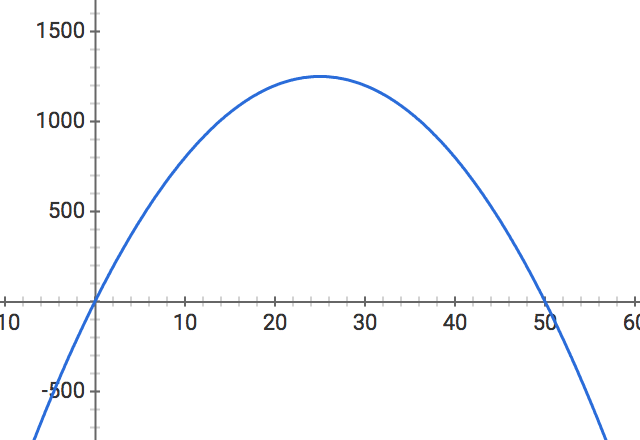
\includegraphics[scale = .5]{images/fence_graph.png}
    \end{center}
}

\frame{
    Algebraic magic:

    $$A(x) = x(100 - 2x) = -2(x - 25)^2 + 1250$$ \pause

    Since 

    $$-2(x - 25)^2 \leq 0$$ \pause

    we get

    $$A(x) \leq 1250$$

    with equality if and only if $x = 25$
}

\frame{
    How does the algebraic magic work? \pause

    \bigskip

    Start with an expression of the form $x^2 + bx$. \pause

    \begin{center}
        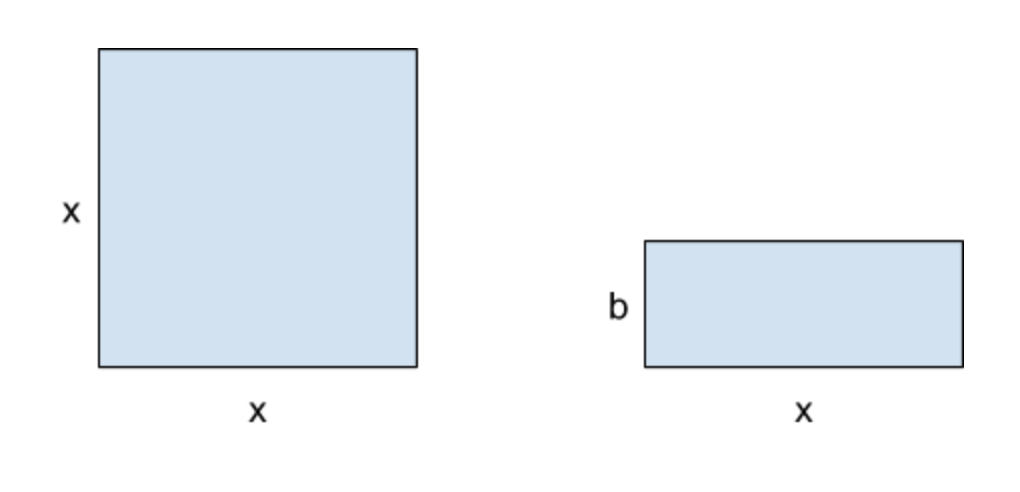
\includegraphics[scale = .5]{images/complete_square1.png}
    \end{center}
}

\frame{
    Cut the $bx$ rectangle in half and rearrange: \pause

    \begin{center}
        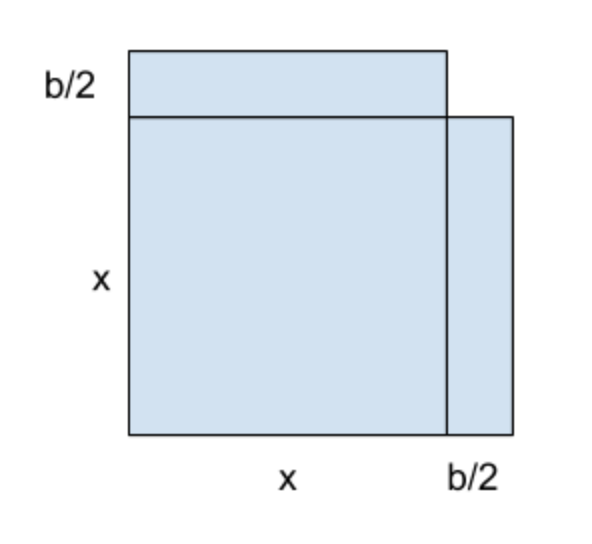
\includegraphics[scale = .5]{images/complete_square2.png}
    \end{center}
}

\frame{
    Complete the square! \pause

    \begin{center}
        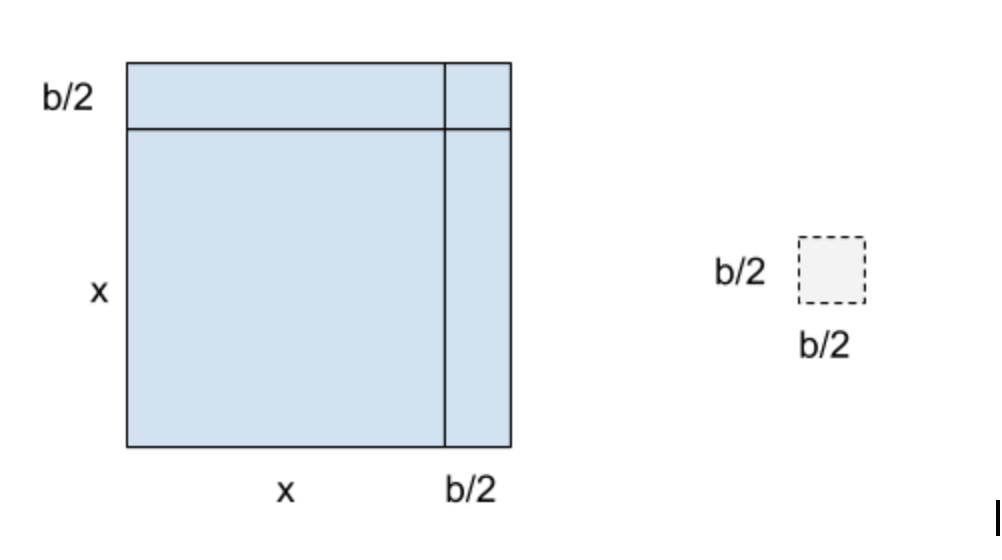
\includegraphics[scale = .5]{images/complete_square3.png} \pause
    \end{center}

    Conclusion:

    $$x^2 + bx = \left( x + \frac{b}{2} \right)^2 - \left(\frac{b}{2}\right)^2$$
}

\frame{
    Let's apply the algebraic magic to the function $A(x) = x(100 - 2x)$ which computes the area of our fence. \pause

    \bigskip

    To do so, we need to find an expression of the form $x^2 + bx$; the first step is to expand the parentheses: \pause

    $$A(x) = x(100 - 2x) = 100x - 2x^2 = -2x^2 + 100x$$ \pause

    Now factor out a $-2$: \pause

    $$A(x) = -2x^2 + 100x = -2(x^2 - 50x)$$
}

\frame{
    Finally, apply the algebraic magic to the expression $x^2 + 50x$, leaving the $-2$ on the outside: \pause

    $$A(x) = -2(x^2 - 50x) = -2((x-25)^2 - 25^2)$$ \pause

    Conclude with a little bit of simplifying:

    $$A(x) = -2(x-25)^2 + 2 \cdot 25^2 = -2(x-25)^2 + 1250$$
}

\frame{
    Let's look at another optimization problem:

    \bigskip

    You want to build an open box with a square base which holds $25m^3$ of water.  How much material do you need?
}

\frame{
    Space of models: \pause

    \begin{\itemize}
        \item Each box is determined by the width $x$ of the base and the height $y$ \pause
        \item Constraints: $x \geq 0$, $y \geq 0$, $\text{Volume} = x^2y = 25$
    \end{itemize}
}

\frame{
    Objective function: \pause

    \bigskip

    The amount of material needed is determined by the surface $S(x,y) = x^2 + 4xy$ of the box.
}

\frame{
    Constrained optimization problem: minimize $S(x,y) = x^2 + 4xy$ subject to the constraints $x \geq 0$, $y \geq 0$, and $x^2 y = 25$. \pause

    \bigskip

    The objective function is quadratic, but the constraint $x^2 y = 25$ is cubic, so we expect this to be harder.
}

\frame{
    Use the constraint to eliminate $y$ and get: \pause

    $$S(x) = x^2 + \frac{100}{x}$$ \pause

    \begin{center}
        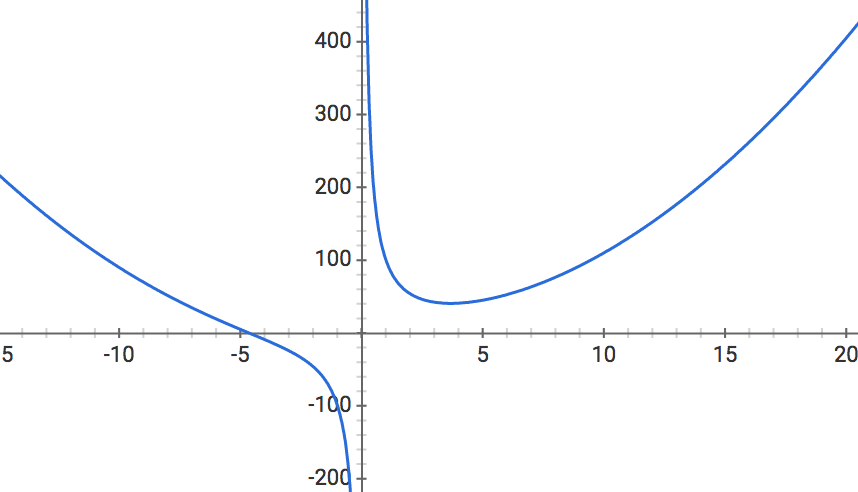
\includegraphics[scale = .5]{images/open_box_graph.png}
    \end{center}
}

\frame{
    No algebraic magic; we'll need some tools. \pause

    \bigskip

    Main idea: approximate a general function with linear and quadratic functions.
}

\frame{
    \frametitle{1.2 Optimization via linear approximation}
    Our objective now is to solve optimization problems of the following form:

    \bigskip

    Find the maximum and/or minimum value of a function $f: A \to \R$ where $\R$ is the set of all real numbers and $A$ is a subset of $\R$. \pause

    \bigskip

    This problem is completely hopeless in general, but there are lots of techniques which work in special cases which come up in applications.
}

\frame{
    In this seminar we'll solve optimization problems by using calculus to understand the geometry of the graph of $f$. \pause

    \bigskip
    
    Assume that $f$ is defined on an interval (or finite collection of intervals) in $\R$; we will look at:

    \begin{itemize}
        \item The \textit{local behavior} of $f$ near points of interest in the interior of its domain \pause
        \item The \textit{boundary behavior} of $f$ near the endpoints of its domain
    \end{itemize}
}

\frame{
    \begin{definition}
        A point $x_\max \in A$ is said to be a \textit{local maximum} for $f$ if 
        
        $$f(x_{\max}) \geq f(x)$$
        
        for all $x$ sufficiently close to $x_\max$.

        Similarly, $x_\min$ is said to be a local minimum if $f(x_{\min}) \leq f(x)$ for all $x$ near $x_{\min}$. 
    \end{definition}
}

\frame{
    To find local extrema, we will use \textit{local linear approximations}. \pause
    
    \bigskip

    Main idea: if $x_0$ is a local extremum of $f$ and $f$ can be well approximated by a line near $x_0$ then that line is flat (has slope zero).
}

\frame{
    \frametitle{1.3 Lines}
    Before approximating functions by lines, let us review some basic facts about them.
}

\frame{
    \begin{definition}
        A function $L$ is said to be \textit{linear} if it satisfies the following conditions:

        $$L(x + y) = L(x) + L(y), \quad L(ax) = a L(x)$$

        for every $x$, $y$, and $a$.
    \end{definition} \pause

    \bigskip

    Fact: every linear function $L \colon \R \to \R$ has the form $L(x) = mx$ for some constant $m$ called the \textit{slope} of $L$.
}

\frame{
    \begin{definition}
        A function $\ell$ is said to be \textit{affine} if the $\ell(x) - b$ is a linear function for some constant $b$, called the \textit{intercept} of $\ell$.
    \end{definition} \pause

    \bigskip

    Every affine function $\ell \colon \R \to \R$ has the form $\ell(x) = mx + b$ for some constants $m$ and $b$. \pause

    \bigskip

    Fact: a function $\R \to \R$ is affine if and only if its graph is a line, and any non-vertical line is the graph of some affine function. \pause

    \bigskip

    It is standard to simply refer to an affine function as a line and write its equation as $y = mx + b$.
}

\frame{
    Given a point $(x_0, y_0)$ in the plane and a slope $m$, one can construct a line which passes through $(x_0, y_0)$ with slope $m$ by solving the following equation for $y$:

    $$y - y_0 = m(x - x_0)$$ \pause

    \begin{example}
        Find a line with slope $-2$ which passes through the point $(3,5)$.
    \end{example}
}

\frame{
    Given two points $(x_0, y_0)$ and $(x_1, y_1)$ in the plane (not on the same vertical line), one can construct a line which passes through both points by using the slope:

    $$m = \frac{y_1 - y_0}{x_1 - x_0}$$ \pause

    \begin{example}
        Find a line which passes through the points $(1, 4)$ and $(7, 5)$.
    \end{example}
}

\frame{
    \frametitle{1.4 Linear approximation and limits}
    When we speak of a linear approximation to a function $f(x)$ at a point $a$, our hope is to find an affine function $\ell(x)$ whose values are as close as possible to the values of $f$ near $a$. \pause

    \bigskip

}

\frame{
    Such a linear approximation does not necessarily exist:
}

\frame{
    Assuming it does exist, how would we find it? \pause

    \bigskip

    Certainly it should pass through the point $(a, f(a))$, so if we can find the slope $m$ then the line has the form
    
    $$y = f(a) + m(x - a)$$
}

\frame{
    Look at the slope of the line passing through $(a, f(a))$ and $(x, f(x))$ for $x$ close to $a$:

    $$m = \frac{f(x) - f(a)}{x - a}$$ \pause

    In some cases it is clear what happens as $x$ gets closer and closer to $a$; for instance, take $f(x) = x^2$: \pause

    \begin{align*}
        \frac{f(x) - f(a)}{x - a} &= \frac{x^2 - a^2}{x - a} \\
                                  &= \frac{(x - a)(x + a)}{x - a} \\
                                  &= x + a
    \end{align*} \pause

    So as $x$ approaches $a$ the slope approaches $a + a = 2a$.
}

\frame{
    Thus part of the fundamentals of linear approximation lies in the notion of a \textit{limit}. \pause

    \bigskip

    Informally, we say that a function $g$ approaches a number $m$ as $x$ approaches a point $a$, written

    $$\lim_{x \to a} g(x) = m$$

    provided that the values of $g$ can be made arbitrarily close to $m$ by restricting the inputs $x$ to some neighborhood of $a$.
}

\frame{
    This definition is admittedly a little vague, but it is possible to make it completely rigorous and to organize all of the theory in this course around the precise definition of a limit. \pause

    \bigskip

    However, scientists and mathematicians happily used calculus to solve hard problems for over two centuries before the rigorous definition was discovered, so we will follow their lead in this seminar and reason from intuition when it is necessary to work with limits.
}

\frame{
    \begin{definition}
        \begin{itemize}
            \item The \textit{derivative} of a function $f$ at a point $a$ is the number

                $$f'(a) = \lim_{x \to a} \frac{f(x) - f(a)}{x - a}$$

                if the limit exists.
                In this case $f$ is said to be \textit{differentiable} at $a$. \pause

            \item If $f$ is differentiable at $a$ then the \textit{local linear approximation} of $f$ at $a$ is the function

                $$\ell(x) = f(a) + f'(a)(x - a)$$
        \end{itemize}
    \end{definition}
}

\frame{
    Intuition: $f'(a)$ represents the factor by which $f$ stretches tiny intervals centered at $a$: \pause
}

\frame{
    \begin{example}
        Use the previous definition to compute the local linear approximation of the given function at the given point.

        \begin{itemize}
            \item $f(x) = x^2$, $a = 2$ \pause
            \item $f(x) = \sqrt{x}$, $a = 4$ \pause
            \item $f(x) = \frac{1}{x}$, $a = 1$
        \end{itemize}
    \end{example}
}

\frame{
    \frametitle{1.5 Computing derivatives}
    Did you struggle a little with $\sqrt{x}$ and $\frac{1}{x}$?
    
    Imagine trying $\frac{x^5}{\sqrt{4x^2 - 7}}$! \pause

    \bigskip

    There are a number of handy rules for recovering the derivative of a complicated function from the derivatives of simpler pieces, and this is normally how one handles functions like the above.
}

\frame{
    \frametitle{Power functions}
    For $p \neq 1$, the derivative of $f(x) = x^p$ is given by

    $$f'(x) = p x^{p - 1}$$ \pause

    \bigskip

    \begin{example}
        \begin{itemize}
            \item Differentiate $f(x) = x^3$ \pause
            \item Differentiate $f(x) = \frac{1}{x^3}$ \pause
            \item Differentiate $f(x) = \sqrt[3]{x}$
        \end{itemize}
    \end{example}
}

\frame{
    \frametitle{Linearity}
    Given $f(x) = a g(x) + b h(x)$ we have

    $$f'(x) = a g'(x) + b h'(x)$$

    if $g$ and $h$ are differentiable at $x$. \pause

    \bigskip

    \begin{example}
        Differentiate $f(x) = x^3 + \frac{2}{x^3} - 4\sqrt[3]{x}$
    \end{example}
}

\frame{
    \frametitle{Chain rule}
    Let $f = h \circ g$, meaning $f(x) = h(g(x))$.  Then:

    $$f'(x) = g'(x) h'(g(x))$$

    if $g$ is differentiable at $x$ and $h$ is differentiable at $g(x)$. \pause

    \bigskip

    Intuition: if $g$ stretches by a factor of $m$ near $x$ and $h$ stretches by a factor of $n$ near $h(x)$ then $g \circ h$ stretches by a factor of $m n$.
}

\frame{
    \begin{example}
        \begin{itemize}
            \item Differentiate $f(x) = (x - 5)^2$ \pause
            \item Differentiate $f(x) = \frac{1}{x^3 + 2x}$ \pause
            \item Differentiate $f(x) = \sqrt[3]{x^2 + 1}$
        \end{itemize}
    \end{example}
}

\frame{
    \frametitle{Product rule}
    Given $f(x) = g(x) h(x)$, we have:

    $$f'(x) = g(x) h'(x) + g'(x) h(x)$$

    if $g$ and $h$ are differentiable at $x$. \pause

    \bigskip

    Intiuition:
}

\frame{
    \begin{example}
        \begin{itemize}
            \item Differentiate $f(x) = (x - 5)^2 (x - 2)^5$ \pause
            \item Differentiate $f(x) = \frac{\sqrt{x}}{x + 2}$
        \end{itemize}
    \end{example}
}

\frame{
    \frametitle{Quotient rule}
    Given $f(x) = \frac{g(x)}{h(x)}$, we have:

    $$f'(x) = \frac{g'(x) h(x) - g(x) h'(x)}{h(x)^2}$$

    if $g$ and $h$ are differentiable at $x$ and $h(x) \neq 0$. \pause

    \bigskip

    \begin{example}
        \begin{itemize}
            \item Differentiate $f(x) = \frac{x^2}{\sqrt{x - 1}}$. \pause
            \item Differentiate $f(x) = \frac{x^5}{\sqrt{4x^2 - 7}}$.
        \end{itemize}
    \end{example}
}

\end{document}
